\chapter{Project Development}
	
In each of the previous chapters I have explored different aspects of the fields of home automation and voice assistance from a 
theoretical point of view, from their definition to smaller details, including additional explanations about a specific home automation 
system, openHAB.

At this time, I think I have provided enough background to begin my case study: the building of a home automation controller. As I 
mentioned in the openHAB chapter, I will base my project on this system and build on it, as it accomplishes very well the main
requirements that I determined for this project.

In this chapter, I will detail the process that I have followed in order to develop this project, from its specification to the final result.

\section{Product Specification}
The first task to do is to define the product. What should a home automation system do? What do users expect it to do? How? All 
the answers to these questions can be clarified by following some processes that, although they do not completely answer them (we 
can see many failed projects from time to time), they provide a very clear and detailed specification from the beginning.

\subsection{Personas}
Creating personas is a common process applied to the product design and development process in order to help in making a user-centered
design, and it is applicable in this project in order to have a better idea of what would users expect from the final product.

A persona is a representation of a user, typically based off user research and incorporating user goals, needs, and interests.

In this project, I am going to use proto-personas, which are based on secondary research and the guess of who they should be designed 
for, as currently we do not have means and time for making true research-based personas (and it is not the main objective in this project).

After thinking about the main uses of this system and the people that would be interested on it, I have extracted these three personas, 
representing its main uses, although not the only ones. I have built them with the online platform Xtensio, and the figures
\ref{fig:persona-oswald-douglas}, \ref{fig:persona-anna-lahtinen} and \ref{fig:persona-rosario-vera} represent them. I tried to extract 
a varied range of backgrounds, current situations, desires and worries. 

Oswald Douglas (figure \ref{fig:persona-oswald-douglas}) is a freelance technology blogger from Dallas, USA, that is very interested 
in the areas of home automation and Internet of Things. He is looking to automate his own home and write about his experience in 
his blog. He already has experience with technology, and this next step will not be too difficult for him. His interests are clear: 
to try cutting-edge technology in his own home and make the most of home automation.

Anna Lahtinen (figure \ref{fig:persona-anna-lahtinen}) is a 16 year-old high school student from Lappeenranta, Finland. She is up 
to date on technology but she is not passionate about it. However, she heard about home automation and thinks that she could enjoy 
a better media experience with it. In addition, she thinks that adding smart color light bulbs to her bedroom would make it look more 
beautiful. However, she feels that there is a lack of general information about devices and the set up and configuration of a home 
automation system. She thinks that the price of it is too high as well.

Rosario Vera (figure \ref{fig:persona-rosario-vera}) is an administrative from Vitoria-Gasteiz, Spain. She is 37 years old, is married and 
has two young children. She is not very familiar with technology, but she has heard about home automation in the news and thinks 
that it could fit her needs. Rosario and her husband work outside home, and sometimes their children need to be alone at home. Home 
automation would provide more security to the home and would allow them to have more spare time. Voice assistance would be helpful 
for their children when they are alone, as it is a very easy and natural way to interact with technology. However, she is concerned about 
their privacy regarding these systems and she thinks that companies should give more accessible explanations about it. In addition, 
she finds these systems difficult to use.

\begin{sidewaysfigure}
	\centering
	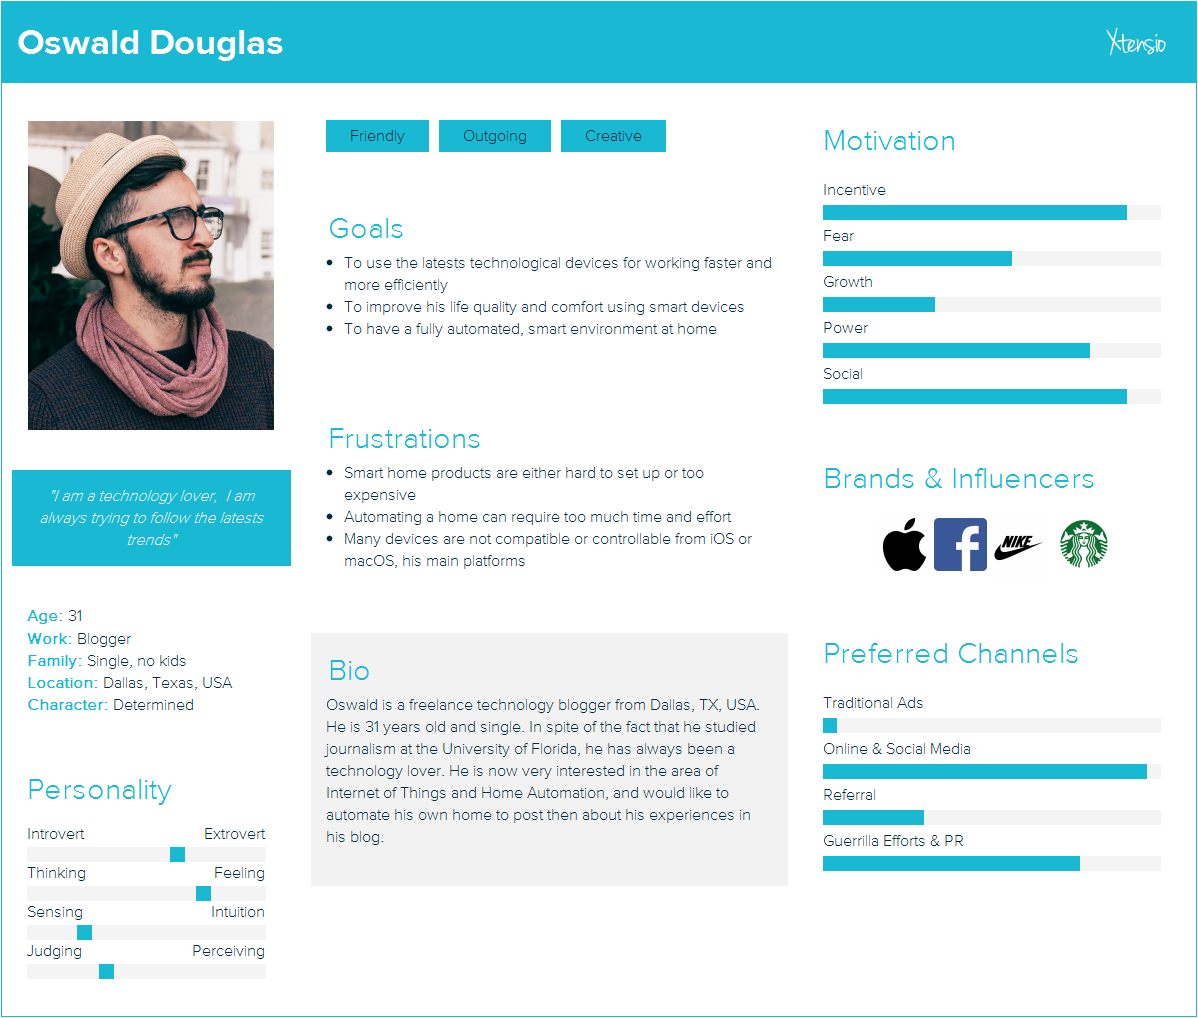
\includegraphics[width=0.65\textwidth]{images/Chapter_06/persona-oswald-douglas.png}
	\caption{Persona: Oswald Douglas}
	\label{fig:persona-oswald-douglas}
\end{sidewaysfigure}

\begin{sidewaysfigure}
	\centering
	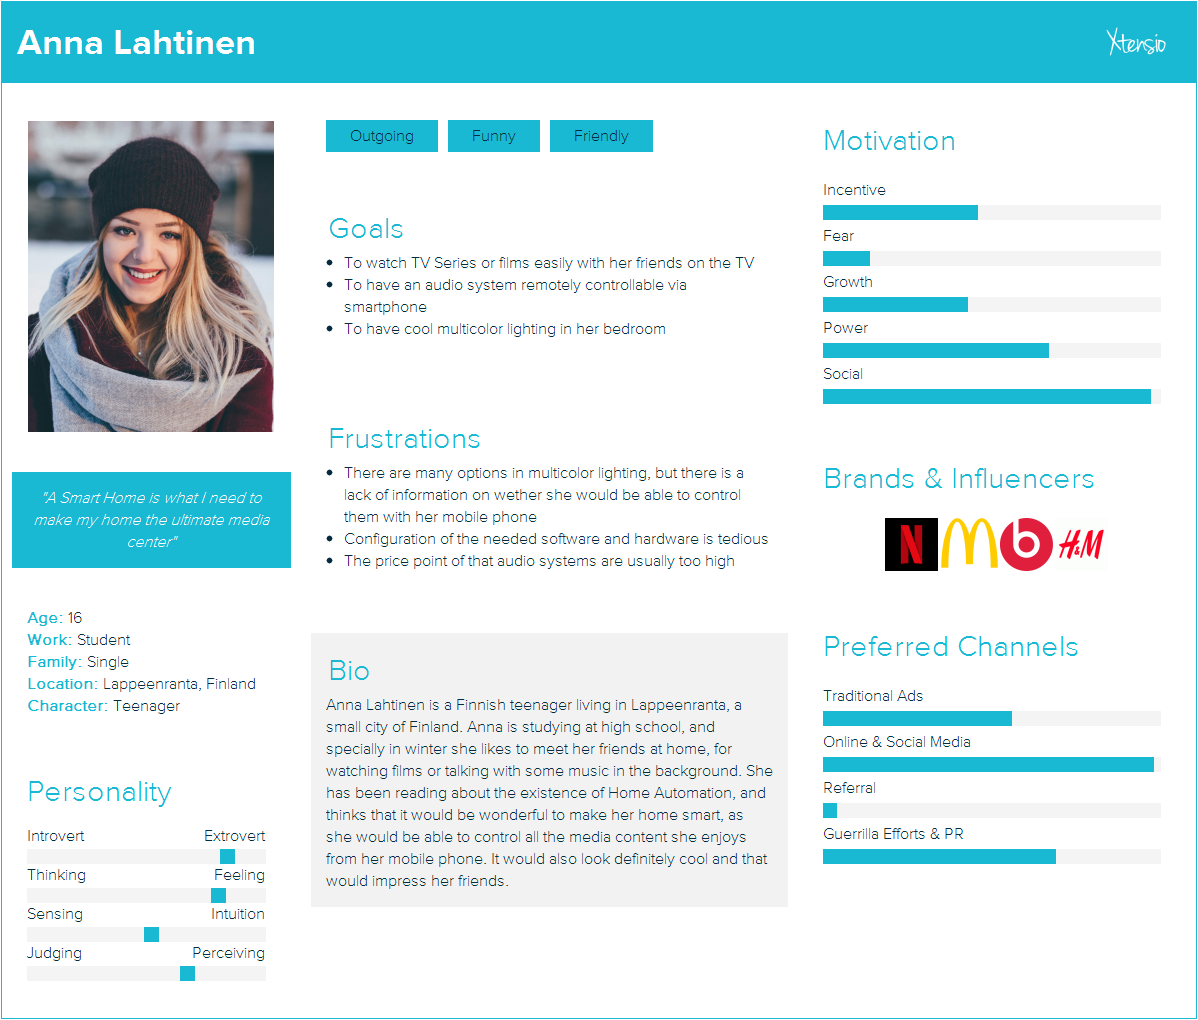
\includegraphics[width=0.65\textwidth]{images/Chapter_06/persona-anna-lahtinen.png}
	\caption{Persona: Anna Lahtinen}
	\label{fig:persona-anna-lahtinen}
\end{sidewaysfigure}

\begin{sidewaysfigure}
	\centering
	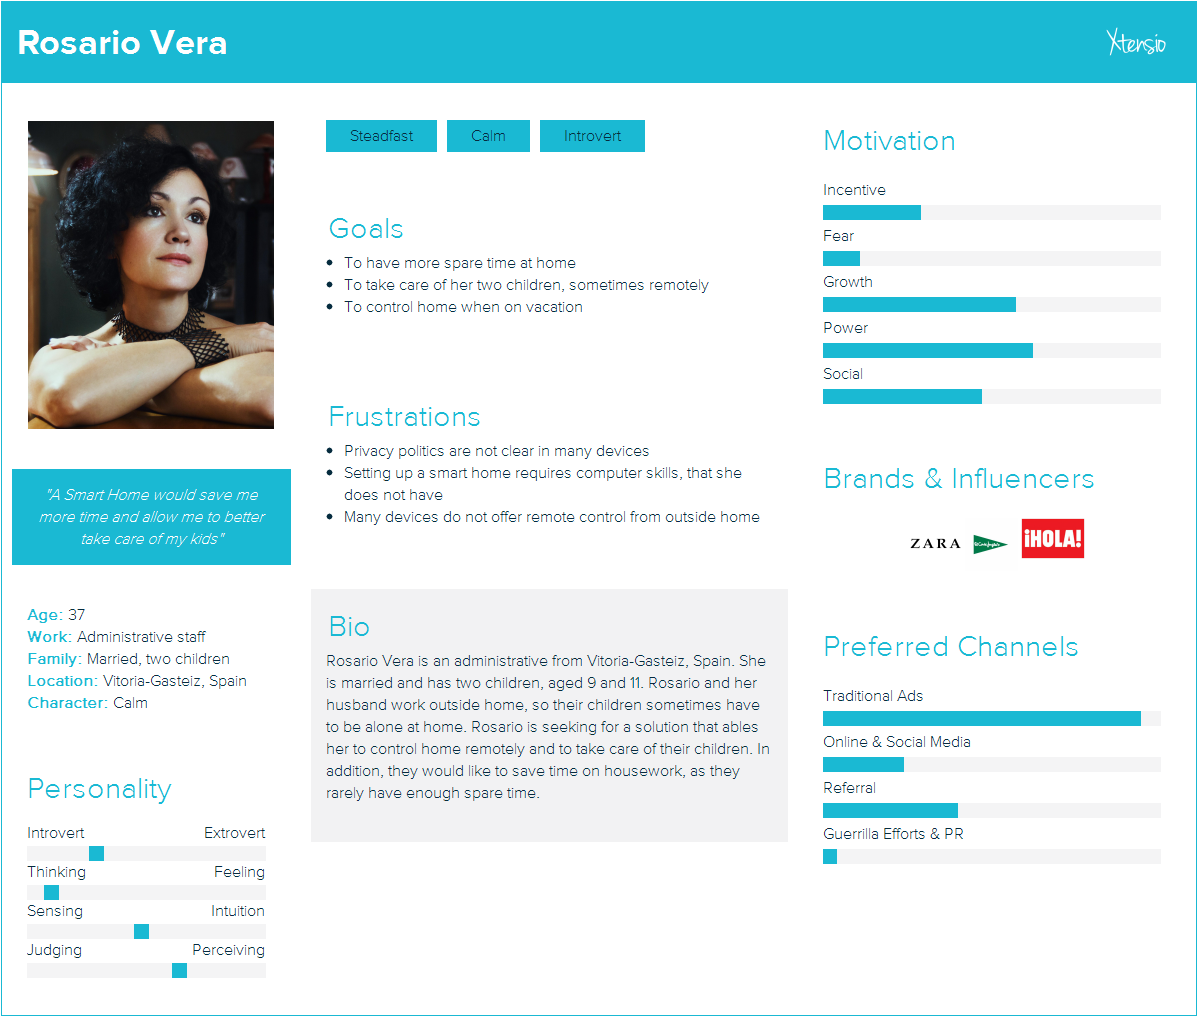
\includegraphics[width=0.65\textwidth]{images/Chapter_06/persona-rosario-vera.png}
	\caption{Persona: Rosario Vera}
	\label{fig:persona-rosario-vera}
\end{sidewaysfigure}

\subsection{Software Requirements Specification}
With the Software Requirements Specification (SRS), I try to describe the project to develop from a functional point of view, that is,
to determine the capabilities that the software system will have.

The domotic controller will be able to control all modern devices in our home, regardless of their maker and the technology they use.
It will provide an easy to use user interface and the ability to easily install, modify or remove the devices. It will also include natural
human-computer interaction through the voice. A more detailed specification of the requirements can be found in the subsections
below.

\subsubsection{Functional Requirements}
Functional requirements are a description of the facility or feature required. They deal with what the system should do or provide 
for users.\cite{sqaFunctionalNonFunctional}

\begin{itemize}
	\item \textbf{FR1}: The system will be able to retrieve automatically the status of the different properties of the elements.
	\item \textbf{FR2}: The system will be able to retrieve automatically data from its different data providers.
	\item \textbf{FR3}: The system will not need any operation to launch openHAB after it is powered on.
	\item \textbf{FR4}: The system will be able to turn itself off safely.
	\item \textbf{FR5}: The system will automatically detect new smart devices connected to the local network.
	\item \textbf{FR6}: The system will be able to detect the possible operations with each connected smart device. 
	\item \textbf{FR7}: The system will be able to operate with the connected devices according to the detected possible operations.
	\item \textbf{FR8}: The system will be able to tell the user in an understandable manner the current connection status for each
	device.
	\item \textbf{FR9}: The system will provide different user interfaces, so users can choose one between them, according to
	their needs.
	\item \textbf{FR10}: The user will be able to change the configuration of the system from a graphical user interface.
	\item \textbf{FR11}: The system will be manually configurable and modifiable using configuration files.
	\item \textbf{FR12}: The system will automatically include and configure new devices found in the network, after the user decides
	to add them.
	\item \textbf{FR13}: The user will be able to configure the name, display icon, IP and all possible aspects of the item directly from
	the user interface.
	\item \textbf{FR14}: The system will allow the user to make groups of items.
	\item \textbf{FR15}: The system will allow the user to add groups of items to other groups of items.
	\item \textbf{FR16}: The system will be modular and include a package system. Each package supports a set of devices.
	\item \textbf{FR17}: The package system will be accessible from the graphical user interface.
	\item \textbf{FR18}: The installation of packages will be done automatically after the user clicks on the install button.
	\item \textbf{FR19}: The removal of packages will be done automatically after the user clicks on the remove button.
	\item \textbf{FR20}: The system will maintain an updated and classified list of packages according to an external repository.
	\item \textbf{FR21}: The system will be manageable from external sources.
	\item \textbf{FR22}: The system will be accessible from external devices and from the Internet.
	\item \textbf{FR23}: The system will allow to have automation rules defined by the user.
	\item \textbf{FR24}: The voice assistant will allow to perform the main operations of each device in the system.
	\item \textbf{FR25}: The voice assistant will be able to answer in different languages.
	\item \textbf{FR26}: The voice assistant will be able to do power management tasks in the system, such as powering the system
	off or restarting the system.
	\item \textbf{FR27}: The voice assistant will be operable through mechanical methods or by voice.
	\item \textbf{FR28}: The users will be able to edit and adapt the functionalities of the voice assistant according to their needs.
	\item \textbf{FR29}: The voice assistant will provide spoken feedback if there has been an error performing the given command.
	\item \textbf{FR30}: The voice assistant will be able to print debug information in the command line if it is required.
\end{itemize}

\subsubsection{Non-Functional Requirements}
Non-functional requirements detail constraints, targets or control mechanisms for the new system. They describe how, how well or
to what standard a function should be provided.\cite{sqaFunctionalNonFunctional}

\begin{itemize}
	\item \textbf{NFR1}: The system, along with the voice assistant, will be installable in the Raspberry Pi.
	\item \textbf{NFR2}: The system and the voice assistant will provide a satisfactory response rate.
	\item \textbf{NFR3}: The user interfaces of the home automation system will be adaptable to the size and resolution of the
	user's screen.
	\item \textbf{NFR4}: The user interfaces will be made according to modern standards, like Material Design.
	\item \textbf{NFR5}: The home automation system will run in a local server, created in the machine which executes it.
	\item \textbf{NFR6}: In order to allow external connections, the home automation system will provide a REST API.
	\item \textbf{NFR7}: The system will provide secure access options.
	\item \textbf{NFR8}: The system must be available the 99\% of the time.
	\item \textbf{NFR9}: The system must be scalable.
	\item \textbf{NFR10}: The system must be recoverable in less than 45 minutes.
	\item \textbf{NFR11}: The cost of the system must me minimal.
	\item \textbf{NFR12}: The system must be interoperable with multiple devices.
	\item \textbf{NFR13}: The voice assistant will recognize English.
	\item \textbf{NFR14}: The voice assistant will be fast in its response. Therefore, its procedure for deciding a response will 
	be optimal.
	\item \textbf{NFR15}: The voice assistant will operate with the home automation system via REST, so it can be installed in a
	different computer than the one with the home assistant.
\end{itemize}

\subsection{Use Cases}
The next step after the specification of requirements is to specify the use cases of the system.

Use case diagrams are usually referred to as behavior diagrams used to describe a set of actions (use cases) that some system or 
systems (subject) should or can perform in collaboration with one or more external users of the system (actors).\cite{umlUseCaseDiagrams}

%TODO
%Hacer los diagramas de casos de uso tal y como indiqué en UC-device-and-service-control.xml
%Dividir los requisitos de modo que queden subsistemas funcionales diferenciados

\subsection{Functional Subsystems}
%TODO
%Especificar aquí los subsistemas funcionales

\subsection{Implementation Possibilities}
After exploring what users would expect from a system like this, it is worth thinking about how it should be implemented. Together 
with my director, I proposed different options to meet the previous requirements.

\subsubsection{Web Platform}
A well designed web platform is a great idea nowadays. If this platform is hosted in a local server, it means that it can be accessed
from any device connected to the network. With the correct configuration, it could be even reachable from anywhere in the world.
It is easy to implement and maintain, and users with basic web development knowledge would be able to easily modify it. In addition,
the same web platform can be adaptable to any device and resolution, thanks to responsive designs. It would also work if we attach
a tactile screen to the Raspberry Pi.

OpenHAB mounts a web platform in a local server by default, and provides several adaptable user interfaces, so this solution would
not require much effort, and it offers many possibilities.

\subsubsection{Desktop Application}
Another solution, focused on the Raspberry Pi desktop (where we mainly want to implement the system), is developing a desktop 
application with an adapted user interface for tactile screens. The advantage of a desktop application is that it usually requires 
less resources and it is faster, but it is a specific solution for the Raspberry Pi, so it would only work there. We would need a 
different application if we wanted it to run on mobile phones or tablets.

We would need to make it from scratch, as openHAB does not provide any desktop application.

\subsubsection{Mobile Application}
Mobile phones and \textit{tablets} are common devices that are widely used to manage smart homes. Some setups have a tablet located 
somewhere in the home, which is only used for managing the domotic devices. An application is faster and more accessible than a web
platform, and users are more used to them, so it would be convenient in some cases.

However, making the system only accessible from a mobile or tablet application would reduce the utility of the Raspberry Pi, and 
would at least require two devices (one for the local server and another one for accessing it). Although it is a good complement to the
system, it is not convenient to base it only on a mobile application. However, it is applicable in a hybrid solution.

\subsubsection{Hybrid Solution}
A hybrid solution consists of applying two or more solutions together of those specified above. For example, providing a web platform 
and an optional mobile application to easily manage the system from a mobile device.

OpenHAB provides a web platform, as explained above, and a mobile application for iOS and Android than connects to the web platform.

\subsubsection{Comparison}
The table \ref{table:possible-implementations} compares all the possibilities for the implementation of the system.

\begin{table}[]
	\centering
	\resizebox{\textwidth}{!}{%
		\begin{tabular}{|l|c|c|c|c|}
			\hline
			\multicolumn{1}{|c|}{\textbf{Feature}}                                  & \textbf{\begin{tabular}[c]{@{}c@{}}Web\\ platform\end{tabular}} & \textbf{\begin{tabular}[c]{@{}c@{}}Desktop \\ application\end{tabular}} & \textbf{\begin{tabular}[c]{@{}c@{}}Mobile\\ application\end{tabular}} & \textbf{\begin{tabular}[c]{@{}c@{}}Hybrid\\ Solution\end{tabular}} \\ \hline
			\begin{tabular}[c]{@{}l@{}}Support for \\ multiple devices\end{tabular} & Yes                                                             & Only PCs                                                                & \begin{tabular}[c]{@{}c@{}}Only mobile\\ phones/tablets\end{tabular}  & Yes                                                                \\ \hline
			\begin{tabular}[c]{@{}l@{}}Allows access\\ from Internet\end{tabular}   & Yes                                                             & No                                                                      & No                                                                    & Yes                                                                \\ \hline
			\begin{tabular}[c]{@{}l@{}}Control from\\ Raspberry Pi\end{tabular}     & Yes                                                             & Yes                                                                     & No                                                                    & Yes                                                                \\ \hline
			\begin{tabular}[c]{@{}l@{}}Easy \\ implementation\end{tabular}          & Yes                                                             & No                                                                      & No                                                                    & Yes                                                                \\ \hline
			\begin{tabular}[c]{@{}l@{}}Maximum\\ performance\end{tabular}           & No                                                              & Yes                                                                     & Yes                                                                   & Partially                                                          \\ \hline
		\end{tabular}%
	}
	\caption{Comparison between possible implementations}
	\label{table:possible-implementations}
\end{table}

As we can see, the hybrid solution, which is a web platform and mobile application, meets all the features in the best way, and 
offers easy and fast implementation. At this point, I have not considered the implementation of the voice assistant, which I will 
talk about in following sections.

\bigskip
\section{System Analysis}
%TODO
%Introducir la sección

\subsection{Conceptual Model}
%TODO
%Especificar el modelo conceptual

\bigskip
\section{System Design}
%TODO
%Introducir la seccion

\subsection{Architecture}
%TODO
%Especificar la arquitectura del sistema, se puede hacer una explicacion rapida de los subsistemas que lo componen

\subsection{Conceptual Class Diagram}
%TODO
%Introducir y especificar el DCC

\bigskip
\section{Implementation}
In this section, I will explain the process that I have followed to implement the home automation controller, along with the voice
assistant.

\begin{figure}
	\centering
	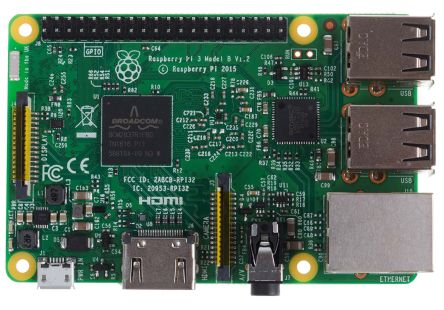
\includegraphics[width=0.8\textwidth]{images/Chapter_06/raspberry-pi-3b.jpg}
	\caption{Raspberry Pi 3 Model B}
	\label{fig:raspberry-pi-3b}
\end{figure}

As I have mentioned before, the main objective is to install the system in a Raspberry Pi, which is an affordable and small computer,
with enough power and connectivity options to install a home automation system on it, and even a voice assistant. The possibilities 
of this device are endless: it can work with or without display, and has a special connector to which the user can connect screens, 
microphones, speakers and many other accessories. It also has USB ports on its high-end models, and accepts all the USB 
accessories that a normal computer would accept.\cite{raspberryPiDocs}

The first approach to this system was to install Raspbian, a Linux distribution provided by openHAB, over a Raspberry Pi 3 Model B 
(figure \ref{fig:raspberry-pi-3b}). Raspbian has openHAB preinstalled and configured, so it is ready to use. The first idea was to 
have a computer with openHAB and then a voice assistant in other machine. I installed the distribution on this mini PC, but after 
reviewing the possible voice assistants, I found that it was not the best way to implement it. 

I found the Google AIY Voice Kit, which is a kit provided by Google to makers that want to play around with voice recognition.
They provide a package with some accessories for the Raspberry Pi and a cardboard box that is meant to contain the board and the
accessories. Then, I reconsidered the architecture. It would be also possible to install openHAB in the same machine as the virtual
assistant. This way, we would need just one machine for all. It would be a voice assistant, but with a local server, accessible from
all the devices connected to the local network. It would be possible to attach a screen to it as well, so the user can manage the
smart home graphically from the same device.

I thought this would be the best solution, and it would still meet all the requirements specified previously. So, I began working on it.

\subsection{Introduction to Google AIY Voice Kit}
The AIY Voice Kit is a do-it-yourself project created by Google that demonstrates how easy and inexpensive can be to create a natural 
voice recognizer that works with Google Assistant, at a price of only EUR 30 in Europe. The project, aimed for makers, also lets the 
user add their own questions, which is the most powerful part for our purpose. 

The idea is to adapt the device in order to fetch the voice commands that the microphone captures and manage them in OpenHAB, 
making the system act following user’s instructions.

\subsubsection{Capabilities}
The main advantage of the Google AIY Voice Kit, and the reason why we have chosen it for this project, is that we can access the 
Google Cloud Voice API and create our own voice interfaces. Everything is coded in Python, and we can create voice commands to 
control it.

This, along with the more than reasonable quality of its stereo microphone and speaker, make it a very useful device that could 
perfectly fit in a smart home, despite its looks.

The device is capable of recognizing the “OK Google” command, as well triggering the assistant when the big red button is pressed, 
and, by default, it is capable of doing almost everything that the Google Assistant on smartphones can do, including integration 
with the apps in the user’s smartphone and reading the news, among other things.

\subsubsection{The Main Challenge}
The challenge is to explore how Google AIY Voice Kit and OpenHAB 2, both installed on the same system, can work together and, 
if it is possible, connect them so a standard user can control its smart home using voice commands and universal, open source solutions.

\subsection{Building the Google AIY Voice Kit}
For making the voice recognizer, I primarily used:

\begin{itemize}
	\item Cardboard for the body of the device.
	\item A speaker.
	\item A Voice HAT microphone board and an accessory board.
	\item A big button with a light inside to trigger the voice recognition.
	\item A Raspberry Pi Model 3 B.
	\item An 8GB microSD card.
	\item Cables to connect everything.
\end{itemize}

\begin{figure}
	\centering
	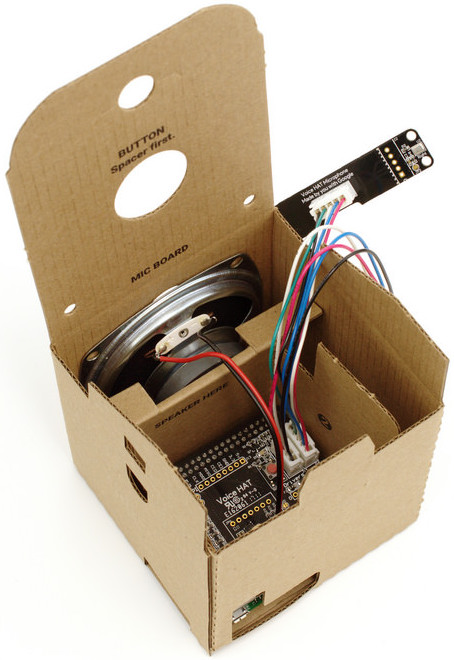
\includegraphics[width=0.5\textwidth]{images/Chapter_06/aiy-voice-kit.jpeg}
	\caption{The AIY Voice Kit}
	\label{fig:aiy-voice-kit}
\end{figure}

First of all, I had to put all the items together and assemble the cardboard body. The Voice HAT accessory board is connected to the 
Raspberry Pi through its GPIO connector, which is adapted to connect the rest of devices: the speaker, the microphone board and the
button. Once everything was correctly connected, I had to assemble the cardboard body, which was composed by two 
pieces.\cite{aiyProjectsVoice}

The next step was to write the Voice Kit SD image\cite{voiceKitSdImage} to the microSD card. I used the \textit{Etcher.io} macOS 
application for this purpose. 

The system includes everything that the Raspberry Pi needs to use the connected devices, so I only needed to check that they worked 
fine and were correctly connected. The system also includes two demos with Google Assistant: one that triggers the assistant by saying 
“OK Google!”, and another that needs the button to be pressed to trigger it.

To make any demo or a new app that uses Google Assistant work, it is necessary to register a new project on Google Cloud Platform 
(GCP) first. A project of this kind has to include the Google Assistant API, which can be enabled via GCP, as well as an OAuth 2.0 
client. Finally, at the moment of running the application, it seeks a JSON file that contains all this information. By default, it 
must be placed in the home folder and it must be called assistant.json.

Google Assistant gathers all the user’s information from their Google account, so they must have enabled the web and app activity, 
the device information and the voice and audio activity from their Activity Controls panel in their Google account settings.

\subsection{Setting up openHAB 2}
In this case, the goal is to install openHAB in the Linux distribution that the AIY Kit provides, which is a fork of Raspbian 
(that is a fork of Debian made for the Raspberry Pi), with the suitable drivers in order to support all the accessories from the kit. 
Luckily, openHAB provide in their documentation pages\cite{openHABDocs} enough instructions to make this process easier.

In this process, I used a keyboard and a mouse for interacting with the operating system, but it can also be done remotely via 
SSH connection.

As a prerequisite, Java 8 must be installed on the system. Users may prefer Zulu, the main Java \textit{alternative}, a fully 
certified build of OpenJDK.\cite{zuluWebsite}

OpenHAB 2 can be installed though a package repository or manually from file, but it is recommended to install through a package
repository, using \textit{apt}, \textit{apt-get}, \textit{yum} or \textit{dnf}. As this operating system is based on Debian, I used 
\textit{apt-get}.

First of all, I have to add the openHAB 2 Bintray repository key to the package manager and allow \textit{apt} to use the HTTPS 
Protocol.

\begin{lstlisting}[style=Consola]
wget -qO - 'https://bintray.com/user/downloadSubjectPublicKey?username=openhab' | sudo apt-key add - 
sudo apt-get install apt-transport-https
\end{lstlisting}

OpenHAB offers Stable (Official), Beta and Snapshot builds to choose from. The stable builds contain the latest official release 
with tested features, so it is the \textit{safest} to use. I will install this one. Then, I need to add the openHAB 2 Stable Repository 
to your systems apt sources list

\begin{lstlisting}[style=Consola]
echo 'deb https://dl.bintray.com/openhab/apt-repo2 stable main' | sudo tee /etc/apt/sources.list.d/openhab2.list
\end{lstlisting}

Next, I have to resynchronize the package index:

\begin{lstlisting}[style=Consola]
sudo apt-get update
\end{lstlisting}

And now I can install openHAB:

\begin{lstlisting}[style=Consola]
sudo apt-get install openhab2
\end{lstlisting}

Optionally, it is possible to install the add-ons package (\textit{openhab2-addons}), but it is meant to be installed if the machine 
is going to be disconnected from the Internet, as openHAB downloads them on request by default. In this case, I assume that the
system is going to be connected to Internet always.

At this point, I can start openHAB and register it to be automatically executed at system startup. To this end, the documentation 
provides the following commands for systems based on \textit{systemd}, such as Raspbian.

\begin{lstlisting}[style=Consola]
sudo systemctl start openhab2.service
sudo systemctl status openhab2.service

sudo systemctl daemon-reload
sudo systemctl enable openhab2.service
\end{lstlisting}

After some minutes, openHAB is ready on the local server, in the port 8080 (accessible in http://localhost:8080). Then, the following
commands are used to control the service.

\begin{figure}
	\centering
	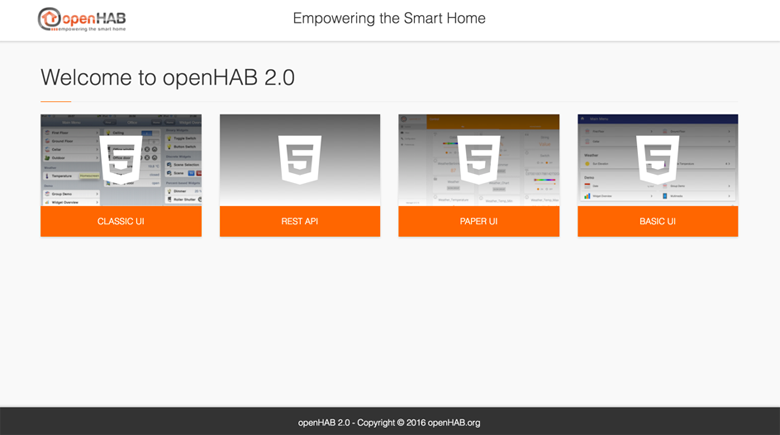
\includegraphics[width=1\textwidth]{images/Chapter_06/openhab-startup.png}
	\caption{OpenHAB 2 startup screen}
	\label{fig:openhab-startup}
\end{figure}

\begin{lstlisting}[style=Consola]
# Current service status
sudo /etc/init.d/openhab2 status

# (Re-)Start openHAB (background service)
sudo /etc/init.d/openhab2 restart

# Stop the openHAB background service
sudo /etc/init.d/openhab2 stop

# Make openHAB automatically start after booting the Linux host
sudo update-rc.d openhab2 defaults
\end{lstlisting}

OpenHAB installs also a utility in the command line interface, named \textit{openhab-cli}, that provides access to the openHAB-specific 
commands.

\begin{lstlisting}[style=Consola]
Usage:  openhab-cli command [options]

Possible commands:
  start [--debug]     -- Starts openHAB in the terminal.
  stop                -- Stops any running instance of openHAB.
  status              -- Checks to see if openHAB is running.
  console             -- Opens the openHAB console.
  backup [filename]   -- Stores the current configuration of openHAB.
  restore filename    -- Restores the openHAB configuration from a backup.
  showlogs            -- Displays the log messages of openHAB.
  info                -- Displays distribution information.
\end{lstlisting}

Lastly, to stay up to date to new releases, they recommend to execute the following commands periodically. Note that this also applies
to the rest of the packages installed in the Linux system.

\begin{lstlisting}[style=Consola]
sudo apt-get update
sudo apt-get upgrade
\end{lstlisting}

\subsection{Adding Philips Hue Devices}
Now that we have openHAB 2 up and running in the Raspberry Pi integrated in the AIY Kit, it is desirable to add a device to the home 
automation system. We have a Philips Hue lightning system available, so in this section I will explain the process that we have followed
to add it and configure it in our openHAB 2 instance.

\subsubsection{The Hue System}
Our Philips Hue system is composed by the \textit{white and color ambiance starter kit}\cite{philipsHueMeethue} (which consists 
in three Hue white and color lights and a Hue hub) as well as a Hue motion sensor:

\begin{itemize}
	\item \textbf{The Hue Hub} acts as a bridge between the user interface (the smartphone application or the OpenHab instance) and 
	the connected devices. It is configured and controlled via the Hue app and supports up to 50 lights at the same time. It communicates 
	via Zigbee with the Hue devices.
	\item \textbf{The Hue Motion Sensor} can be configured to turn on and off the lights when it detects movement and under some 
	defined conditions. By default, it is configured from the Hue app.
	\item \textbf{The Hue White and Color Lights} are customizable RGB lights. By default, they are configurable from the Hue app, 
	which offers many ways of changing the light emission.
\end{itemize}

\subsubsection{Installation and Configuration Process on PaperUI}
Philips, as many other companies, is restrictive regarding their home automation devices, and every communication between the Hue 
devices and the controller (openHAB in this case) needs to pass through the Hue Hub. The Hub communicates via WiFi with the controller 
and via Zigbee with the Hue devices. The software it uses is privative, but luckily openHAB 2 implements protocols that make possible 
the communication between the controller and the Hub. This makes the Hub, though, a frustrating addition to our home automation system.

The Hue system needs to be configured from the Philips Hue mobile application in the first place. This process will link the Hub with the 
desired Hue devices, so the next time that the user connects to the Hub, it will not be necessary to configure them again, even if 
the connection is done from openHAB. The application allows to manage rooms and sort the devices, as well as setting automated commands 
(for instance, turning the light on when the motion sensor detects any movement). OpenHAB is unable to perform such complex operations 
by default, providing only a few channels for the light bulb.

Once the Hub is on, connected and linked with the Hue devices, we can proceed to configure it on OpenHAB. In this case, I explain 
the process to follow in order to add the light bulb controls, but it might work for other Hue devices in a future. If OpenHAB is 
used on a system connected to the same network as the Hub, the Hub will automatically appear in the \textit{Inbox} section. We have 
to make sure before that its related binding. Adding the Hub in the Inbox section means that it will be listed as a Thing. OpenHAB 
takes care automatically of the Thing (figure \ref{fig:philips-hue-hub-thing}) and Items configuration. After adding them, the host 
device and the Hub will be able to communicate between them. However, the user needs to press the pairing button on the Hub in 
order to activate the communication.

\begin{figure}
	\centering
	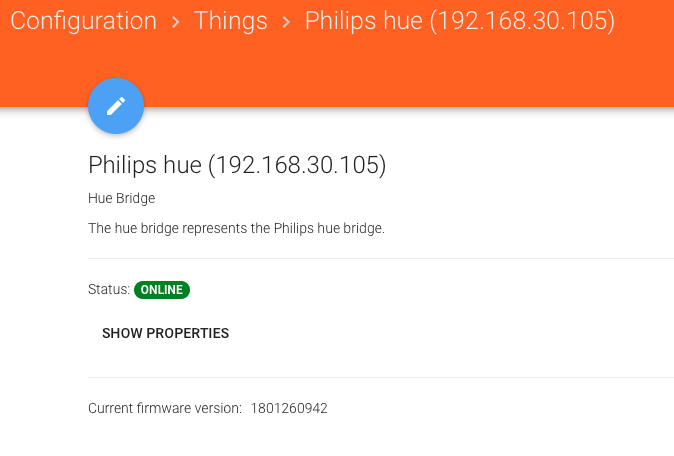
\includegraphics[width=0.9\textwidth]{images/Chapter_06/philips-hue-hub-thing.png}
	\caption{Philips Hue Hub Thing}
	\label{fig:philips-hue-hub-thing}
\end{figure}

After that, the Hub will act as a bridge and openHAB will be able to display all the compatible devices connected to the Hub. In 
this case, the Hue color lamp appears in the Inbox. The process for adding it is the same as with the Hub. Nevertheless, this time 
the light controls will be added automatically to the Control panel according to the linked channels on the thing. OpenHAB supports 
two channels that are directly related to the bulb functionality: \textit{color} (which is divided in tone, brightness and saturation) 
and \textit{white temperature}. The first one will set the light in a color with the desired properties, and the second will set a 
white color from a range of whites (from cold to warm white). Additionally, OpenHAB provides two more channels: \textit{alert}, 
to use the bulb as an alert light under certain circumstances, and \textit{color loop}, which will make the light color iterate in 
the whole color spectrum. The figure \ref{fig:hue-color-bulb-channels} shows the PaperUI interface showing these channels.

\begin{figure}
	\centering
	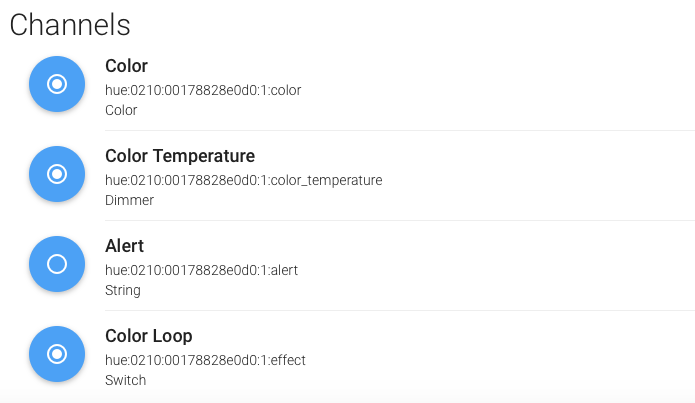
\includegraphics[width=0.9\textwidth]{images/Chapter_06/hue-color-bulb-channels.png}
	\caption{Available channels in the Hue color bulb}
	\label{fig:hue-color-bulb-channels}
\end{figure}

\begin{figure}
	\centering
	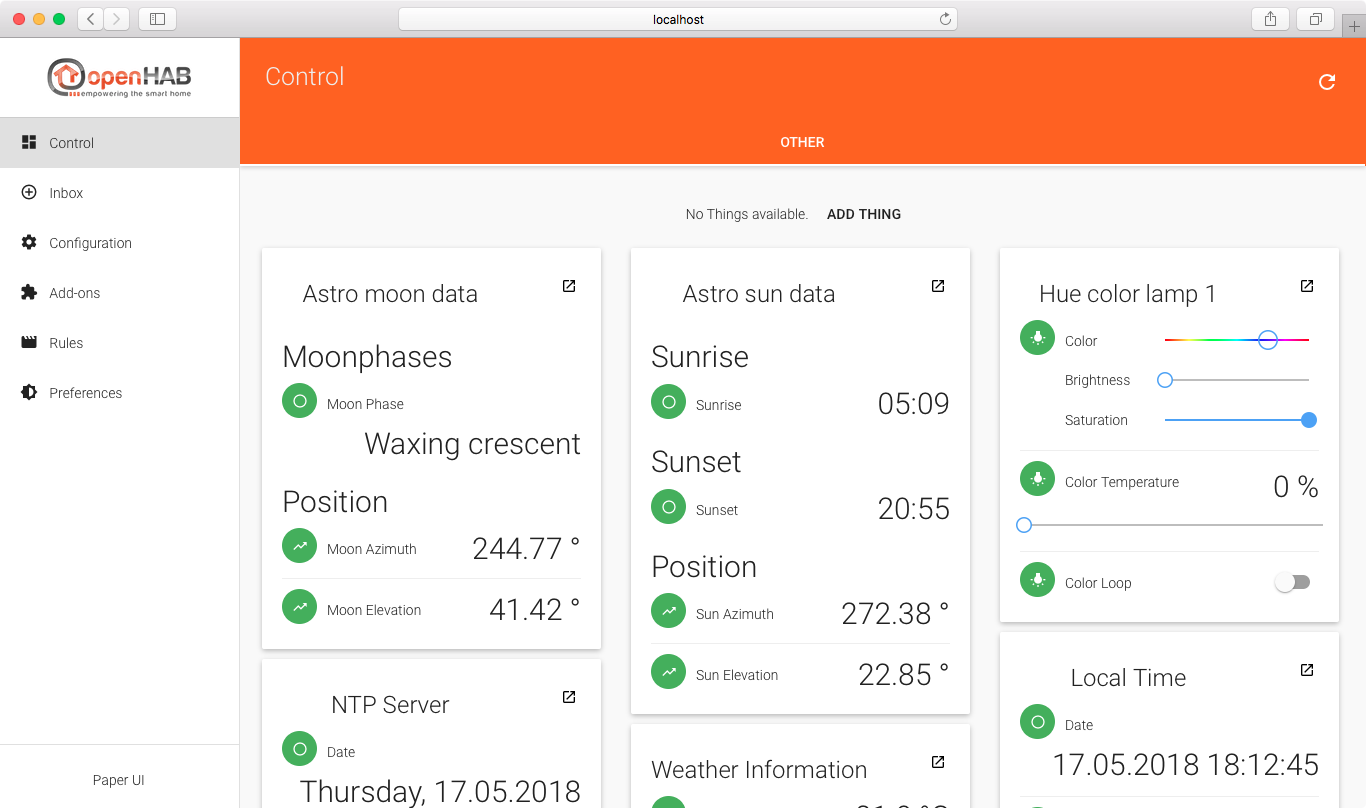
\includegraphics[width=1\textwidth]{images/Chapter_06/openhab-control-hue.png}
	\caption{OpenHAB 2 Control Panel with the Hue color bulb controls}
	\label{fig:openhab-control-hue}
\end{figure}

\subsubsection{Internal Functionality}
OpenHAB is able to communicate with the Hue Hub and Hue devices thanks to the Philips Hue binding (represented as a set of packages 
in Java, as shown in the figure \ref{fig:hue-binding-structure}), integrated in the Eclipse SmartHome Extensions repository. 

\begin{figure}
	\centering
	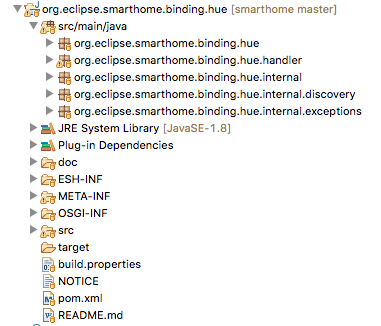
\includegraphics[width=0.6\textwidth]{images/Chapter_06/hue-binding-structure.png}
	\caption{Philips Hue binding internal structure}
	\label{fig:hue-binding-structure}
\end{figure}

As we can see, there are packages for handling the lights and Hub (which is named \textit{bridge}), and for managing the internal 
functionality of the binding and OpenHAB. That is, discovering the devices and showing them in the Inbox and managing exceptions. 
Examples of exceptions can be having the device off or sending the device a wrong command.

Looking more closely at the device handlers, we can see that the bridge handler implements a \textit{Runnable} object with a 
\textit{run} method, which gets the Hub configuration. The function gets the IDs of all the lights connected to the Hub and iterates 
over them. If a light is not listed in a list of light states caught from OpenHAB, it is added as a new light. If it is listed, then 
it checks for changes in the status of the light, comparing the actual state with the last one saved. If the states are different, 
notifies the Light listeners. There is a \textit{LightStatusListener} interface that is called on each change, it will modify the 
Light and Hue objects.

\subsection{Specifying Items Manually}
In previous chapters, I introduced the concept of Item in openHAB 2. Items represent functionalities that can be used by the 
applications, mainly user interfaces or automation logic.

OpenHAB is able to configure many Things and Items automatically in the PaperUI. But in many cases we may need to specify Items
manually. For example, for creating custom views(sitemaps), as we will see below. Therefore, it is important to know how to specify
Items manually.

First of all, I need to create an Items file. Both the items and the sitemap files are located in the \$OPENHAB\_CONF directory, 
which is different on different operating systems. In my case, they are located in:

\begin{lstlisting}[style=Consola]
/usr/share/openhab2/conf/items       <-- *.items files
/usr/share/openhab2/conf/sitemaps    <-- *.sitemap files
\end{lstlisting}

After a fresh installation these directories are empty (except for the \textit{readme} files), so I have to create a file there.
I will call it \textit{default.items}.

OpenHAB has its own syntax for defining Items and Sitemaps, but it is very easy to use. The basic syntax for defining an item is:

\begin{lstlisting}[style=Consola]
ItemType ItemName "ItemDescription" <ItemIcon> {ItemToThingChannelLink}
\end{lstlisting}

The code I have used for defining the item linked to the color channel and the item linked to the white tone channel of a Philips 
Hue color bulb is the following:

\begin{lstlisting}[style=Consola]
Color HueColor1 "Hue Light Bulb 1 Color" <lightbulb> {channel="hue:0210:00178828e0d0:1:color"}

Dimmer HueDimmer1 "Hue Light Bulb 1 Temperature" <lightbulb> {channel="hue:0210:00178828e0d0:1:color_temperature"}
\end{lstlisting}

Now, these Items are registered in the system, but before we can see them, I have to define a sitemap and include them there.

\subsection{Creating a Sitemap}
PaperUI, the newest addition in openHAB 2, is meant to make easier the device management, configuration and discovery. Many of 
these processes are carried out seamlessly, without user intervention. But this user interface lacks some functionalities, such as
custom ordering of Things. \textit{Sitemaps} are custom views that can be displayed in another user interface, the Basic UI, which
is also automatically installed at the beginning.\cite{openHABDocs} Sitemaps take defined Items and display them as the user specifies 
in the UI.

The user is able to define as many sitemaps as desired, and they can be selected from OpenHAB 2 home screen, in the Basic UI. Sitemaps 
are text files with the .sitemap extension, and they are defined in the folder thet I specified in the previous section, inside the OpenHAB 
installation directory.

The basic syntax that a sitemap follows is:

\begin{lstlisting}[style=Consola]
sitemap <sitemapname> label="<title of the main screen>" 
{
    [all sitemap elements]
}
\end{lstlisting}

Sitemaps are composed by arranging various user interface elements. A set of different element types supports a user-friendly and 
clear presentation. One line of Sitemap element definition produces one corresponding UI element. As shown in the example on the
figure \ref{fig:hue-bulb-sitemap}, each element generates a descriptive text next to an icon on the left side and a status and/or 
interaction elements on the right.

A certain set of parameters can be configured to customize the presentation of an element. In the shown example \textit{item} and 
\textit{icon} are parameters. Almost all parameters are optional, some are however needed to result in a meaningful user interface. 

By encapsulating elements with curly brackets, multiple elements can be nested inside or behind others. The Frame element type is 
often used in combination with element blocks. Frames are used to visually distinguish multiple elements of the same topic on one 
interface page. When using code blocks behind other element types such as \textit{Text}, \textit{Group} or \textit{Switch}, these UI 
elements will, in addition to their normal function, be links to a new view, presenting the nested elements. In the example in 
\ref{fig:hue-bulb-sitemap}, I created a single Frame that represented all the functionalities of the Hue Color Light.

The \textit{sitemap} element is mandatory in a Sitemap definition. This element shall be the first line in the sitemap file, and the 
following code block comprises the entire Sitemap definition.\cite{openHABDocs}

\begin{figure}
	\centering
	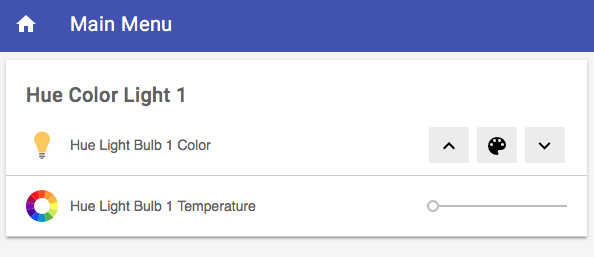
\includegraphics[width=0.9\textwidth]{images/Chapter_06/hue-bulb-sitemap.png}
	\caption{Basic UI displaying a Hue Color Light Item}
	\label{fig:hue-bulb-sitemap}
\end{figure}

From the previous example, I built a sitemap that could display the Hue color light Item that I configured previously in the Basic UI.
The figure \ref{fig:hue-bulb-sitemap} shows the result of introducing the following code in a file that I called \textit{default.sitemap}.

\begin{lstlisting}[style=Consola]
sitemap demo label="Main Menu"
{
    Frame label="Hue Color Light 1" {
        Colorpicker item=HueColor1 icon="slider"
        Slider item=HueDimmer1 icon="colorwheel"
    }
}
\end{lstlisting}

A frame is containing the main functionality of the Hue color light bulb, and that can be done for every new component installed at home.

OpenHAB 2 allows us to group our items so we can sort them by room or type. That can be made through the Group Item type.

\subsubsection{Elements on a Sitemap}
The element types specified in the table \ref{table:openhab-sitemaps-types} may be used in a Sitemap definition file.

\begin{table}[]
	\centering
	\resizebox{\textwidth}{!}{%
		\begin{tabular}{|l|l|}
			\hline
			\multicolumn{1}{|c|}{\textbf{Type}} & \multicolumn{1}{c|}{\textbf{Description}} \\ \hline
			Chart & Adds a time-series chart object for persisted data \\ \hline
			Colorpicker & Allows the user to choose a color from a color wheel \\ \hline
			Default & \begin{tabular}[c]{@{}l@{}}Renders an Item in the default UI representation specified \\ by the type of the given Item\end{tabular} \\ \hline
			Frame & \begin{tabular}[c]{@{}l@{}}Establishes an area containing various other Sitemap \\ elements\end{tabular} \\ \hline
			Group & \begin{tabular}[c]{@{}l@{}}Concentrates all elements of a given group in a nested \\ block\end{tabular} \\ \hline
			Image & Renders an image given by an URL \\ \hline
			Mapview & Displays an OSM map based on a given Location Item \\ \hline
			Selection & \begin{tabular}[c]{@{}l@{}}Provides a dropdown or modal popup presenting values\\ to choose from for an Item\end{tabular} \\ \hline
			Setpoint & \begin{tabular}[c]{@{}l@{}}Renders a value between an increase and a decrease \\ buttons\end{tabular} \\ \hline
			Slider & Presents a value in a progress-bar-like slider \\ \hline
			Switch & Renders an Item as an ON/OFF or multi-button switch \\ \hline
			Text & Renders an Item as text \\ \hline
			Video & Displays a video stream, given a direct URL \\ \hline
			Webview & Displays the content of a webpage \\ \hline
		\end{tabular}%
	}
	\caption{Types of elements for a Sitemap in openHAB 2}
	\label{table:openhab-sitemaps-types}
\end{table}

Data presented by Sitemap elements will almost always originate from a referenced Item. Each Item is of a certain Item type, for 
example \textit{Switch}, \textit{Number} or \textit{String}.

While not all combinations are meaningful, Items of one \textit{datatype} may be linked to different Sitemap element types. This 
provides the flexibility to present Items in the way desired in the home automation user interface.

\bigskip
At this point, I have openHAB installed in the Raspberry Pi inside the AIY Voice Kit. OpenHAB is communicating with the Hue Hub and
the Hue Color Light, and its state can be changed by accessing to the server that openHAB has created in the local network. This means
that, if I type on the browser of my mobile phone the IP address of openHAB and its port (8080), I will be able to control the light from
my phone as well. The state of the bulb can be changed from PaperUI (with the view that it has generated automatically) and from 
Basic UI, with the view and Items that I have specified in these previous steps.

Now the challenge is to build an assistant that can communicate with openHAB, and that is able to change the state of the configured
Items.

\subsection{Voice assistants and Speech-To-Text services}


